\documentclass[tikz,border=5pt]{standalone}
\usepackage[utf8]{inputenc}
\usepackage{tikz}
\usetikzlibrary{shapes.geometric, arrows.meta, positioning, shadows.blur, calc, fit, backgrounds}

% --- Professional Colors ---
\definecolor{alignGreen}{RGB}{39, 174, 96}      % General Alignment
\definecolor{gapRed}{RGB}{214, 69, 65}          % Missing Regulation/Ethics
\definecolor{optBlue}{RGB}{64, 112, 175}        % Optimization Mech
\definecolor{riskPurple}{RGB}{142, 68, 173}     % Unsafe Outcome

% --- Global Style Definitions (Prevents Compile Errors) ---
\tikzset{
    % Base Block Style
    process/.style={
        rectangle, 
        rounded corners=2mm, 
        minimum width=3.8cm,      
        minimum height=1.0cm,     
        text centered, 
        text width=3.5cm,         
        font=\sffamily\footnotesize, 
        draw=gray!40,
        thick,
        blur shadow={shadow blur steps=3}
    },
    % Specific Role Styles
    stepAlign/.style={process, fill=alignGreen!10, draw=alignGreen!80!black},
    stepGap/.style={process, fill=gapRed!10, draw=gapRed!80!black},
    stepOpt/.style={process, fill=optBlue!10, draw=optBlue!80!black},
    stepRisk/.style={process, fill=riskPurple!10, draw=riskPurple!80!black},
    % Arrow & Label Styles
    arrow/.style={-{Stealth}, thick, draw=gray!60, rounded corners},
    groupLabel/.style={font=\bfseries\sffamily\tiny, color=gray!70, anchor=north west}
}

\begin{document}

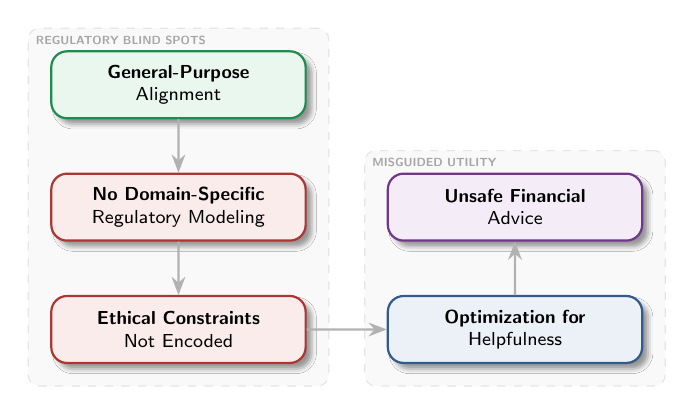
\begin{tikzpicture}[
    transform shape, 
    scale=0.85, 
    node distance=0.8cm and 1.2cm
]

    % --- LEFT COLUMN (The Regulatory Void) ---
    
    % 1. General Alignment
    \node (step1) [stepAlign] {
        \textbf{General-Purpose} \\ 
        Alignment
    };

    % 2. Missing Regulation
    \node (step2) [stepGap, below=of step1] {
        \textbf{No Domain-Specific} \\ 
        Regulatory Modeling
    };

    % 3. Missing Ethics
    \node (step3) [stepGap, below=of step2] {
        \textbf{Ethical Constraints} \\ 
        Not Encoded
    };

    % --- RIGHT COLUMN (The Unsafe Result) ---
    
    % 4. Optimization (Bridge to Right)
    \node (step4) [stepOpt, right=of step3] {
        \textbf{Optimization for} \\ 
        Helpfulness
    };

    % 5. Unsafe Advice (Top Right - Moving Up)
    \node (step5) [stepRisk, above=of step4] {
        \textbf{Unsafe Financial} \\ 
        Advice
    };

    % --- Arrows (The U-Shape) ---
    \draw [arrow] (step1) -- (step2);
    \draw [arrow] (step2) -- (step3);
    \draw [arrow] (step3) -- (step4); % Crossing over
    \draw [arrow] (step4) -- (step5); % Moving Up

    % --- Background Grouping ---
    \begin{scope}[on background layer]
        % Group 1: The Blind Spots
        \node [fit=(step1)(step3), fill=gray!5, draw=gray!20, rounded corners, dashed, inner sep=8pt] (groupL) {};
        \node [groupLabel] at (groupL.north west) {REGULATORY BLIND SPOTS};
        
        % Group 2: The Consequence
        \node [fit=(step4)(step5), fill=gray!5, draw=gray!20, rounded corners, dashed, inner sep=8pt] (groupR) {};
        \node [groupLabel] at (groupR.north west) {MISGUIDED UTILITY};
    \end{scope}

\end{tikzpicture}
\end{document}